\documentclass{article}
\usepackage{natbib}
\usepackage{graphicx}
\usepackage{tabularx}
\usepackage{changepage}
\usepackage{pdflscape}
\usepackage{booktabs}


\usepackage{Sweave}
\begin{document}
\Sconcordance{concordance:supplemental.tex:supplemental.Rnw:%
1 9 1 1 0 86 1 1 8 1 2 19 0 1 2 16 1 1 2 19 0 1 2 49 1}

\title{VALET: \emph{de novo} pipeline for finding metagenomic mis-assemblies}
\author{Supplemental Material}
\date{}
\maketitle
\section{VALET Pipeline}

\begin{figure}
\begin{center}
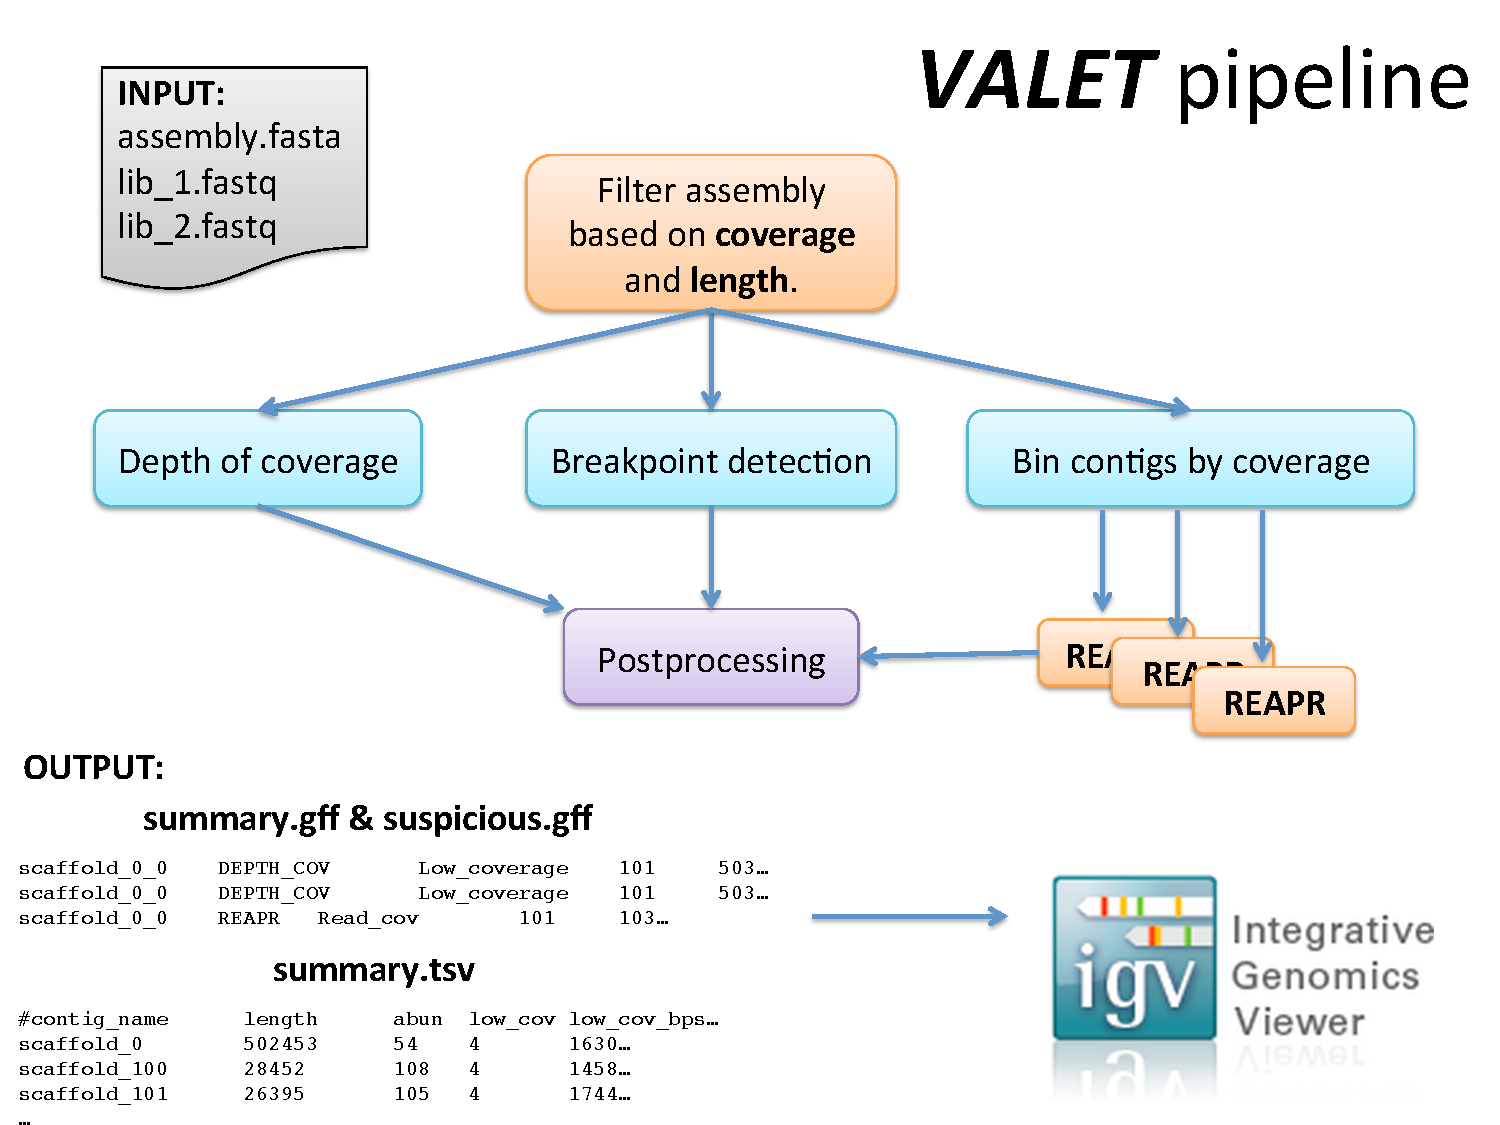
\includegraphics[width=\textwidth]{figures/valet_pipeline}
\end{center}
\caption[valet_pipeline]{Digram of the VALET pipeline.}
\label{fig:valet_pipeline}
\end{figure}

VALET flags regions as potential mis-assemblies when the characteristics of the sequence data do not meet the assumptions for the sequence generation process regarding (1) depth of coverage, (2) insert size consistency, and (3) alignability of the sequences (Figure~\ref{fig:valet_pipeline}). 
Regions that share multiple mis-assembly signatures may be more likely an \textit{actual} mis-assembly.



\subsection{Depth of Coverage Analysis}
The sequencing process of randomly-sheared fragments follows a Poisson distribution~\citep{lander1988genomic}.  Regions within assembled contigs that show high variance in coverage may be potential mis-assemblies. 
Areas of high and low depths of coverage could be compressed/expanded repeats, chimeric contigs, and other types of contamination. 
The main benefit of this approach is that it is completely data-dependent. No prior assumptions of the distribution of the quality values need to be made.

\subsection{Insert size consistency}
Although the sequence technology can only give the raw sequence of the first couple hundred basepairs from the ends of the fragment, the distance between the ends of the sequences can be used to aid in resolving repeats, and orienting and scaffolding contigs. 
Regions of an assembly containing a disproportionate number of mate-pairs (reads from the same fragment) with incorrect insert sizes may be a potential mis-assembly.

\subsection{Identifying assembly breakpoints}
The reads given to the assembler should be alignable to the resulting assembly.
During sequencing, reads are produced starting from random locations within the genome.
Thus, the reads must be able to align to the resulting assembly.
In practice, however, a read may fail to align for a few reasons.
When a read is unable to align to an assembly, there must be some explanation.
In metagenomic samples, an unaligned read can be from a rare, low coverage organism, and was never assembled with any other reads.
A read with a large amount of errors will be unable to align within a specified similarity to the assembly.
A read can come from a unfiltered contaminant or primer.
If a read does not fall into one of the above categories, then it may be a sign of a potential mis-assembly.

\section{Evaluation}
\subsection{Definition of a mis-assembly}
We compared misassemblies identified by VALET on a simulated and synthetic metagenomic dataset to the reference based metagenome assembly evaluation tool MetaQUAST~\citep{mikheenko2015metaquast}.
We ran VALET on the assemblies and compared the errors found with the reference-based mis-assemblies detected by MetaQUAST.
MetaQUAST uses the Plantagora’s definition of a mis-assembly,
i.e., a mis-assembly breakpoint is defined as a position in the assembled contigs where (1) the left flanking
sequence aligns over 1kb away from right flanking sequence on the reference, or (2) the sequences overlap by
over 1kb, or (3) the right flanking sequence aligns on opposite strands or different chromosomes. 
As mutations in the strain in a metagenome can contain structural variants relative to the reference genome. 
MetaQUAST uses the read mapping structural variant caller MANTA~\citep{chen2015manta} to filter canidate misassemblies. 
If any part of a region flagged by VALET overlaps with a mis-assembled region reported by MetaQUAST, we consider it a true positive (mis-assembly correctly identified by our method).
%In addition, the N50 of each assembly is recalculated after breaking at mis-assemblies found by QUAST.

\section{Example Misassembly}
Misassemblies identified by VALET can be further investigated using a genome viewer. the VALET was used to compare metagenome. 
For example, lets look at one of the suspicious regions flagged in an assembly of a Vaginal introitus sample (SRS014465) from the Human Microbiome Project~\citep{human2012structure} (Supplemental Material Figure ~\ref{fig:hmp_plasmid}).
VALET flags a 1.7 kbp high coverage region flanked by breakpoints.
This region BLASTs~\citep{BLAST} to \emph{Lactobacillus amylovorus} GRL 1118 plasmid2 (CP002611.1).
The right flanking region of the contig from positions 5,362 to 10,839 aligns to \emph{Lactobacillus crispatus} ST1, strain ST1 (FN692037.1) with 98\% similarity.
The left flanking ~3.75 kb region does not have a complete alignment with any sequence in NCBI; the closest alignment being from positions 1 to 2,599 to \emph{Lactobacillus helveticus} strain KLDS1.8701 (CP009907.1).

\begin{figure*}
\begin{center}
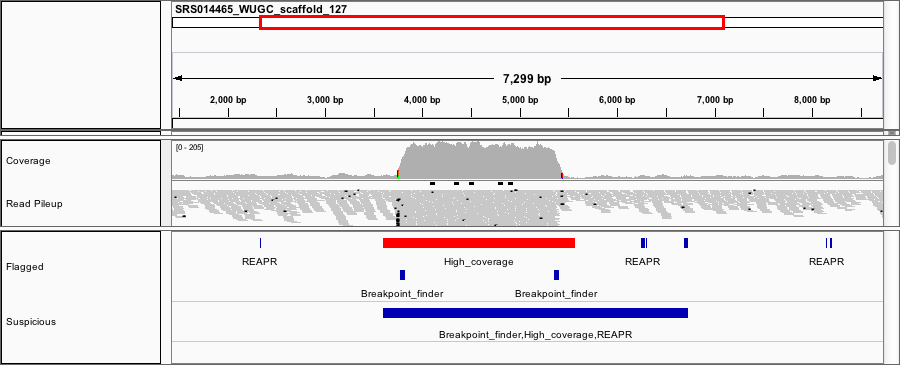
\includegraphics[width=\textwidth]{figures/hmp_plasmid}
\end{center}
\caption[hmp_plasmid]{An example suspicious region flagged by VALET in the HMP assembly of of a Vaginal introitus sample (SRS014465) from the Human Microbiome Project~\citep{human2012structure}.}
\label{fig:hmp_plasmid}
\end{figure*}


\section{Comparison of Valet and MetaQUAST}
%Evaluating correctness – mock even/staggered/mixture of known communities.
%Examining error composition of all HMP data sets.
%Grab a handful to compare with new assemblies.
%Show that window length doesn’t matter when comparing.
%Does window length matter when comparing assemblies.
\subsection{Simple Mock Metagenomic Community}
We examine the overlap in misassemblies identified by VALET and MetaQUST using a simple mock metagenomic community consisting of four bacteria at varying abundances: 80X \emph{Bacteroides vulgatus}  ATCC8482 (Accn. NC\_009614.1), 60X \emph{Bacillus cereus} (Accn. NC\_003909.8), 40X \emph{Actinomyces odontolyticus} (Accn. NZ\_DS264586.1), and 20X \emph{Acinetobacter baumannii} (Accn. NC\_009085.1).
Approximately four million reads are simulated using \textsc{wgsim} ~\citep{li2013wgsim} with default parameters and 100 bp forward and reverse reads.
%% Add text with reference to bash script in github repo
The dataset was assembled with Velvet~\citep{zerbino2008velvet}, MetaVelvet~\citep{namiki2012metavelvet}, MaSuRCA~\citep{zimin2013masurca}, and SOAPdenovo2~\citep{luo2012soapdenovo2} algorithms using MetAMOS~\citep{treangen2013metamos}.
SOME TEXT SUMMARIZING THE COMPARISON RESULTS (Table~\ref{mock_comp_tbl}).  
\subsubsection{NOTES}
This section will be removed later. MetaQUAST does not identify any error for the SOAPdenovo and Velvet assemblies thus no misassemblies for the two assemblers. VALET does however identify misassemblies. The QUAST-VALET comparison tool in VALET does not generate any output when no misassemblies are called by QUAST/MetaQUAST.  



\begin{table}

\caption{VALET results for simulated mock community consisting of four bacteria at varying abundances. Reads were assembled using the four provided assemblers. General assembly statistics include length in Mbp (Len), number of contigs (Ctgs), N50 contig size in kbp (N50), N50 of contigs after broken at mis-assemblies in kbp (NA50) and mismatches per  were calculated for contigs \textgreater 5 kbp. The number of errors detected by MetaQUAST ( MQ Errs), number of flagged regions by VALET (Flg), number of flagged regions that overlap an error found by MetaQUAST (Flg Overlap), number of valid misassemblies or flagged regions with multiple misassembly signatures (Vld), number of valid revions that overlap an error found by MetaQUAST (Vld Overlap).\label{mock_comp_tbl}}
\begin{tabular}{lrrrr}
\toprule
Metric & MaSuRCA & MetaVelvet & SOAPdenovo2 & Velvet\\
\midrule
Len & 16,491,755 & 12,162,955 & 8,317,492 & 1,006,455\\
Ctgs & 343 & 312 & 841 & 149\\
N50 & 83,189 & 67,835 & 10,424 & 6,603\\
NA50 & 81,327 & 65,716 & 10,424 & 6,027\\
MPK & 67.55 & 63.41 & 58.32 & 56.82\\
\addlinespace
MQ Errs & 53 & 20 & 0 & 0\\
Flg & 401 & 165 & 0 & 0\\
Flg Overlap & 41 & 16 & 0 & 0\\
Vld & 33 & 17 & 0 & 0\\
Vld Overlap & 25 & 11 & 0 & 0\\
\bottomrule
\end{tabular}
\end{table}
\subsection{Synthetic Metagenomic Community}

\begin{figure}
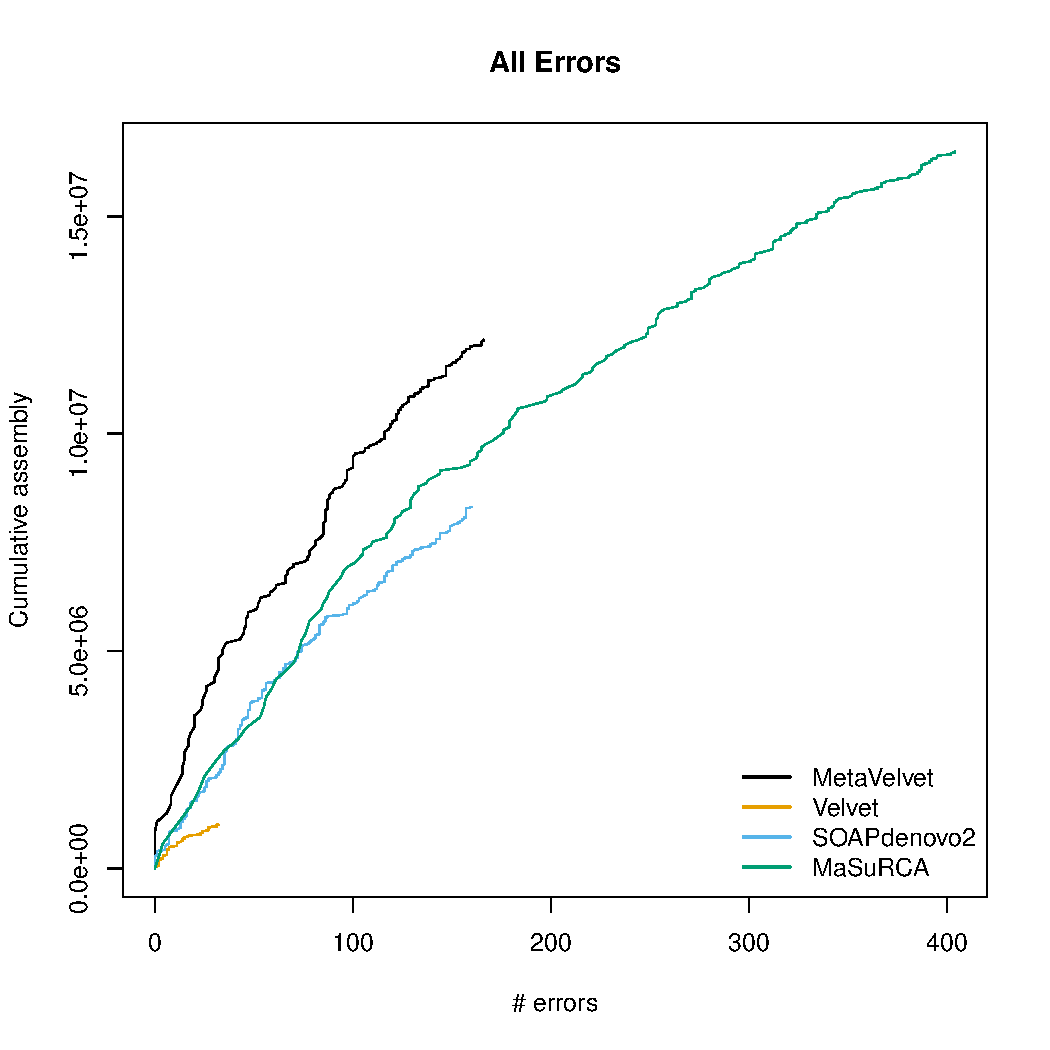
\includegraphics[width=3.86in]{figures/simulated_frc}
\caption[FRC plot of a simulated mock community]{FRC plot provided by VALET of a simulated mock community.}
\label{fig:simulated_frc}
\end{figure}

A major challenge of evaluating assemblies of environmental datasets is that a sizeable portion of the organsisms are unknown or lack a draft genome to compare against.
In silico simulations often lack the complexity and sequencing biases present in real environmental samples.
Fortunately, Shakya et al. provide a \emph{gold standard} synthetic metagenomic dataset containing a mixture of 64 organisms (16 members of Archaea and 48 organisms from 18 Bacteria phyla) with complete or high-quality draft genomes and 200-fold differences in abundances~\citep{shakya2013comparative}.
The dataset consists of 53.4 million reads (101 bp in length).
We assembled the dataset using Velvet~\citep{zerbino2008velvet}, MetaVelvet~\citep{namiki2012metavelvet}, SPAdes~\citep{bankevich2012spades}, and SOAPdenovo2~\citep{luo2012soapdenovo2} by MetAMOS~\citep{treangen2013metamos}.
We ran VALET on the assemblies and compare the errors found with the reference-based mis-assemblies detected by MetaQUAST (Table~\ref{syn_comp_tbl}). 
These rankings match those provided by VALET (Figure~\ref{fig:simulated_frc}).

\begin{table}

\caption{VALET results for assemblies of the Shakya et al.~\citep{shakya2013comparative} dataset. Reads were assembled using the four provided assemblers. General assembly statistics include length in Mbp (Len), number of contigs (Ctgs), N50 contig size in kbp (N50), N50 of contigs after broken at mis-assemblies in kbp (NA50) and mismatches per  were calculated for contigs \textgreater 5 kbp. The number of errors detected by MetaQUAST ( MQ Errs), number of flagged regions by VALET (Flg), number of flagged regions that overlap an error found by MetaQUAST (Flg Overlap), number of valid misassemblies or flagged regions with multiple misassembly signatures (Vld), number of valid revions that overlap an error found by MetaQUAST (Vld Overlap).\label{syn_comp_tbl}}
\begin{tabular}{lrrrr}
\toprule
Metric & MetaVelvet & SOAPdenovo2 & SPADES & Velvet\\
\midrule
Len & 134,157,560 & 150,990,751 & 173,364,620 & 133,773,517\\
Ctgs & 5,707 & 5,782 & 5,367 & 6,042\\
N50 & 41,337 & 50,979 & 74,297 & 36,654\\
NA50 & 38,279 & 45,408 & 62,668 & 33,908\\
MPK & 45.9 & 41.89 & 92.22 & 47.26\\
\addlinespace
MQ Errs & 332 & 472 & 1174 & 327\\
Flg & 1111 & 1288 & 1551 & 1136\\
Flg Overlap & 7 & 18 & 45 & 7\\
Vld & 3 & 3 & 2 & 3\\
Vld Overlap & 0 & 0 & 0 & 0\\
\bottomrule
\end{tabular}
\end{table}



%%%%%%%%%%%%%%%%%%%%%%%%%%%%%%
%% assembly values
%% different assemblies were used in the analysis, not sure if we should update the values or remove the text
%%%%%%%%%%%%%%%%%%%%%%%%%%%%%%
%While the MEGAHIT and Omega assemblies are close in total size (192.3 Mbp vs. 194 Mbp, respectively), MEGAHIT has nearly twice as many contigs as Omega (19,145 vs. 10,284).
%QUAST detects far more mis-assemblies in the Omega assembly compared to MEGAHIT (56,917 vs. 770, respectively).
%VALET detects 34.80\% and 96.10\% of these mis-assemblies found by QUAST in the MEGAHIT and Omega assemblies, respectively.
%While Omega has a higher N50 than MEGAHIT (44.1 Kbp vs. 38.9 Kbp), after breaking at mis-assemblies, the N50 drops well below MEGAHIT's (11.9 Kbp vs. 33.5 Kbp), illustrating why the N50 metric is not always a good indicator of assembly quality.
%VALET is able to accurately assess the quality of the two assemblies without using the reference genomes.

\subsection{Mis-assemblies not validated by MetaQUAST}
One contig, roughly 25 Kbp in size, had a 5 Kbp region at the start of the contig marked as high coverage (Figure~\ref{fig:rrna_coverages}).
This region was roughly 4x the median coverage of the remaining contig.
Using NCBI's BLAST~\citep{BLAST} and reference database, the region aligned to the organism \emph{Nostoc} sp. PCC 7120.
Upon closer inspection, this region contained 16S, 23S, and 5S rRNA genes and was found at \emph{four} locations in \emph{Nostoc} sp. PCC 7120.
This region was only found once in the assembly, so all the sequences from the repeats aligned to this region, inflating the coverage.
This noticeable and consistent increase in coverage caused VALET to mark it as mis-assembled.
Unsurprisingly, QUAST did not mark this as a mis-assembly because the actual sequence within this region matched the reference.

\begin{figure}[tb!]
\begin{center}
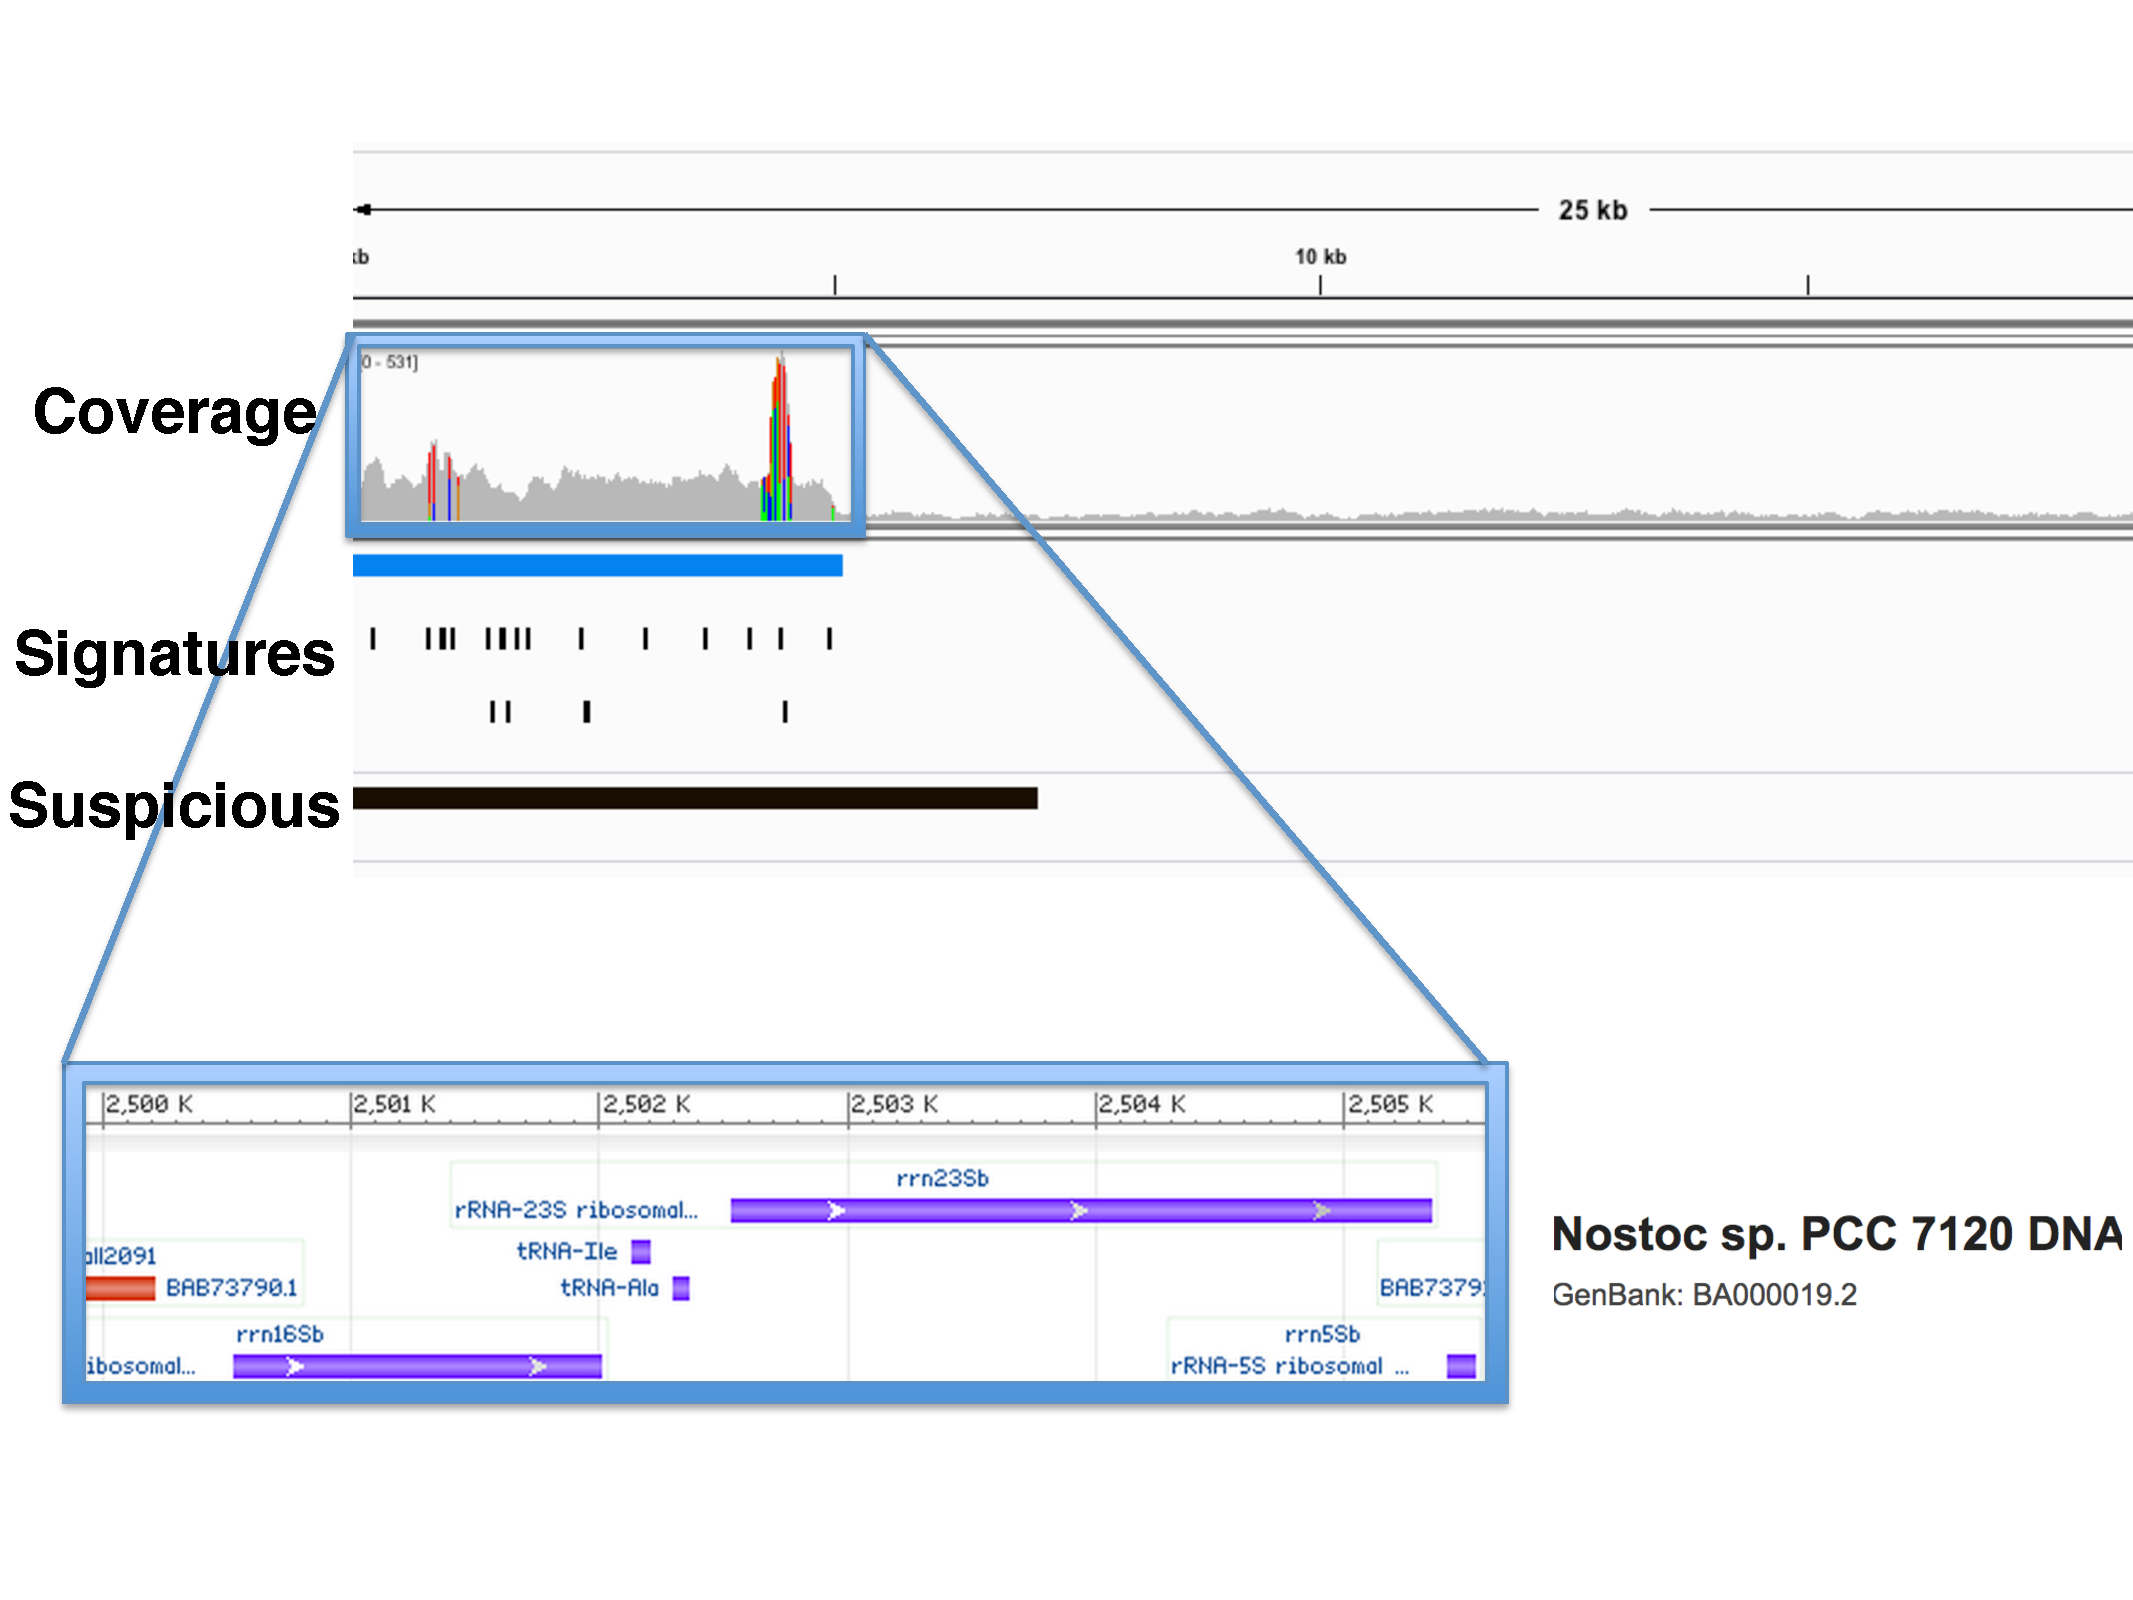
\includegraphics[width=\textwidth]{figures/rrna_coverages}
\end{center}
\caption[16S_rrna]{A closer examination of a region flagged by VALET, but no mis-assembly reported by QUAST. This region contained 16S, 23S, and 5S rRNA genes and was found at four locations in the \emph{Nostoc sp. PCC 7120 genome}.}
\label{fig:rrna_coverages}
\end{figure}


\subsubsection{NOTES}
This section will be removed later. These results are for one of the assemblies not presented in the current results. 
Options are to run re-run VALET on this assembly and make sure VALET identified this misassembly but not MetaQUAST.  Alternatively, present new results using the batch IGV analysis similar to what I did for one of the previous mock datasets.




\bibliographystyle{natbib}
\bibliographystyle{achemnat}
\bibliographystyle{plainnat}
\bibliographystyle{abbrv}
\bibliographystyle{bioinformatics}

%\bibliographystyle{plain}

\bibliography{valet}

\end{document}
